%\newcommand{\node}{%
%  \begingroup\normalfont
%  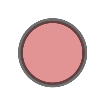
\includegraphics[height=\fontcharht\font`\c]{node.eps}%
%  \endgroup
%}
%
%\newcommand{\threenode}{%
%  \begingroup\normalfont
%  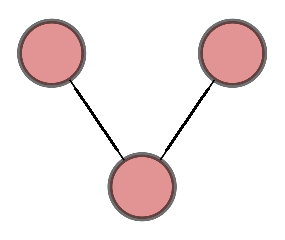
\includegraphics[height=\fontcharht\font`\B]{3nodetree.eps}%
%  \endgroup
%}

\begin{wideslide}[bm=,toc=]{Models of computation}
Different computational models have been developed independently:
\begin{itemize}
\item<2->Turing machines, Alan Turing (covered in CS3101)
\item<3->Lambda calculus, Alonzo Church
\item<4->Post systems, Emil Post
\item<5->and others.
\end{itemize}
\pause[5] Post systems are of interest to us.
\begin{itemize}
\item<7-> They can be used to define something (data structure, program).
\item<8-> Definitions may be recursive \pause[3]

\hspace{2em}$A \equiv \ldots A\ldots$ \pause

or mutually recursive \pause

\hspace{2em}$A \equiv \ldots B\ldots$

\hspace{2em}$B \equiv \ldots A\ldots$

\item<12-> Post systems admit formal proofs---is a definition correct?
\end{itemize}
\end{wideslide}

\begin{wideslide}[bm=,toc=]{Recursive definitions}
A recursive definition can be represented in a {\em Post system\/}.
\begin{itemize}
\item<2-> Named after mathematician Emil Leon Post.
\item<3-> A Post system comprises a finite set of {\em variables\/}, {\em signs\/} and {\em productions\/} 
(inference rules).
\end{itemize}
\pause[3]
An inference rule has the form 
\pause
\begin{displaymath}
\begin{array}{c}
t_1\;t_2\;\cdots\;t_n\\
\hline
t
\end{array}
\end{displaymath}
\pause
where $t,t_1,\ldots ,t_n$ ($n\geq 0$) are terms (strings of signs and variables).
\begin{itemize}
\item<7-> $t_1,\ldots , t_n$ are the {\em antecedents\/}
\item<8-> $t$ is the {\em consequent\/} or conclusion.
\item<9-> When $n=0$, an inference rule is called an {\em axiom\/}.
\end{itemize}
\end{wideslide}

\begin{wideslide}[bm=,toc=]{Recursive definitions}
A Post system of two productions:
\pause
\vspace{-1em}
\begin{tabbing}
{\bf R}XX \=  \kill
{\bf B} \>
        \(\begin{array}[t]{l}
        3\in S
        \end{array}\) \\[2ex]
\pause
{\bf R} \>
        \(\begin{array}[t]{l}
        x \in S \;\;\;y \in S \\
        \hline
        x + y \in S
        \end{array}\)
\end{tabbing}
\pause
The set of signs is $\{3,\in,+\}$ and variables $\{x,y\}$.\\~\\
\pause
\textbf{Claim}: This system defines the set of all positive multiples of 3.
\begin{itemize}
\item<6-> Must prove $n\in S$ iff $n$ is a positive multiple of 3.
\item<7-> ``$n\in S$ only if $n$ is a positive multiple of 3'' (system {\em soundness\/}).
\item<8-> ``$n\in S$ if $n$ is a positive multiple of 3'' (system {\em completeness\/}).
\end{itemize}
\end{wideslide}

\begin{wideslide}[bm=,toc=]{Example derivation showing $9 \in S$}
\vspace{20mm}
\begin{center}
\begin{tabular}{lllll}
  \onslide{2-}{$\bid{B}$  & $\id{3}\in \id{S}$}           & \onslide{3-}{$\id{3}\in \id{S}$ & $\bid{B}$}
  \onslide{4-}{\\ \cline{2-3}}
  \onslide{5-}{$\bid{R}$  & $\id{3} + \id{3} \in \id{S}$} &                    & \onslide{6-}{$\id{3}\in \id{S}$ & $\bid{B}$} 
  \onslide{7-}{\\ \cline{2-4}} 
  \onslide{8-}{$\bid{R}$  & $\id{3} + \id{3} + \id{3} \in \id{S}$ &           & &  \\} 
\end{tabular}
\end{center}

\end{wideslide}
\begin{wideslide}[bm=,toc=]{Recursive Definitions}
A Post system with multiple axioms.
\begin{tabbing}
{\bf R1}XX \=  \kill
\pause
{\bf B1} \>
        \(\begin{array}[t]{l}
        4\in P
        \end{array}\) \\[2ex]
\pause
{\bf B2} \>
        \(\begin{array}[t]{l}
        5\in P
        \end{array}\) \\[2ex]
        
\pause
{\bf R} \>
        \(\begin{array}[t]{l}
        x \in P \;\;\;y \in P \\
        \hline
        x + y \in P
        \end{array}\)
\end{tabbing}
\pause
\textbf{Claim}: every amount of postage at least $12$ can be formed using only $4$
and $5$-cent stamps (Rosen pg. 337).
\begin{itemize}
\item<6-> Must show every positive integer at least $12$ belongs to $P$. 
equal to 12.
\item<7-> This is a completeness result of the system.
\end{itemize}
\end{wideslide}

\begin{wideslide}[bm=,toc=]{Recursive Definitions}
\begin{itemize}
\item  Another Post system with multiple axioms.
\begin{tabbing}
{\bf R1}XX \=  \kill
{\bf B1} \>
        \(\begin{array}[t]{l}
        \epsilon \in \id{Pal}
        \end{array}\) \\[2ex]
{\bf B2} \>
        \(\begin{array}[t]{l}
        a\in \id{Pal}
        \end{array}\) \\[2ex]

 {\bf B3} \>
        \(\begin{array}[t]{l}
        b\in \id{Pal}
        \end{array}\) \\[2ex]
        
{\bf R} \>
        \(\begin{array}[t]{l}
        x \in \id{Pal} \;\;\;y \in \id{Pal} \\
        \hline
        x(yx) \in \id{Pal}
        \end{array}\)
\end{tabbing}
\item Claim:  $\id{Pal}$ defines exactly the set of palindromes over $\{a,b\}^*$.
\end{itemize}
\end{wideslide}

\begin{wideslide}[bm=,toc=]{Recursive Definitions}
\begin{itemize}
\item  A Post system with multiple recursive rules.
\begin{tabbing}
{\bf R1}XX \=  \kill
{\bf B} \>
        \(\begin{array}[t]{l}
        \epsilon \in \id{X}
        \end{array}\) \\[2ex]

{\bf R1} \>
        \(\begin{array}[t]{l}
        x\in \id{X} \\
        \hline
        1x0 \in \id{X}
        \end{array}\) \\[2ex]

{\bf R2} \>
        \(\begin{array}[t]{l}
        x\in \id{X} \\
        \hline
        0x1 \in \id{X}
        \end{array}\) \\[2ex]
       
{\bf R3} \>
        \(\begin{array}[t]{l}
        x \in \id{X} \;\;\;y \in \id{X} \\
        \hline
        xy \in \id{X}
        \end{array}\)
\end{tabbing}
\item Claim: for all $y \in \{0,1\}^*$, $y \in \id{X}$ iff $y$ has an equal
number of $0$s and $1$s.
\item Rule $\bid{R3}$ is needed to show $1001 \in \id{X}$, for instance.
\end{itemize}
\end{wideslide}

\begin{wideslide}[bm=,toc=]{Recursive definitions}
\begin{itemize}
\item A Post system recursively defining the set {\em P\/} of all well-formed formulae in propositional logic:
\begin{displaymath}
\begin{array}{lll}
        \begin{array}[t]{l}
        \bid{T}\in P
        \end{array}
&
        \begin{array}[t]{l}
        \bid{F}\in P
        \end{array}
&
	\begin{array}[t]{l}
        x \in P \\
        \hline
        \neg x \in P
        \end{array} \\[6ex]

	\begin{array}[t]{l}
	x \in P \;\;y \in P \\
	\hline
	x \wedge y \in P
	\end{array}
&
	\begin{array}[t]{l}
	x \in P \;\;y \in P \\
	\hline
	x \vee y \in P
	\end{array}
&
	\begin{array}[t]{l}
	x \in P \;\;y \in P \\
	\hline
	x \Rightarrow y \in P
	\end{array} \\[6ex]

	\begin{array}[t]{l}
        x \in \id{Var} \\
        \hline
        x \in P
        \end{array}
\end{array}
\end{displaymath}
%\item Consequents have larger terms than antecedents except in last rule.
\end{itemize}
\end{wideslide}

\begin{wideslide}[bm=,toc=]{Rooted trees in Rosen 7th Ed.}
  Recall the definition of rooted trees given in Rosen (p. 351).
  
  The set of \emph{rooted trees}, where a rooted tree consists of a set of
  vertices containing a distinguished vertex called the \emph{root}, and
  edges connecting these vertices, can be defined recursively by these steps:
  
  \begin{tabbing}
  {\bf RECURSIVE}XX \=  \kill
  {\bf BASIS} \>
           A single vertex $r$ is a rooted tree.\\[2ex]
  {\bf RECURSIVE} \>
          Suppose that $T_1,T_2,...,T_n$ are disjoint rooted trees with roots\\
  {\bf } \>
          $r_1,r_2,...r_n$, respectively. Then the graph formed by starting with\\
  {\bf } \>
          a root $r$, which is not in any of the rooted trees $T_1,T_2,...T_n$,\\
  {\bf } \>
          and adding an edge from $r$ to each of the vertices $r_1,r_2,...r_n$, \\
  {\bf } \>
          is also a rooted tree.\\[2ex] \\
\end{tabbing}
\end{wideslide}

\begin{wideslide}[bm=,toc=]{Rooted trees}
\begin{itemize}
\item We want a definition amenable to induction---use a Post system instead.
\item Need 3 {\em constructors\/} $\id{cons}$, $\id{node}$ and $\id{nil}$.

\vspace{1em}
\begin{tabular}{|ll|} \hline
{\em integer list\/} & {\em list shorthand} \\ \hline
$\id{nil}$ & $[\;]$ \\
$\id{cons}(3,\id{nil})$ & $[3]$ \\
$\id{cons}(5,\id{cons}(3,\id{nil}))$ & $[5,3]$ \\
$\id{cons}(2,\id{cons}(5,\id{cons}(3,\id{nil})))$ & $[2,5,3]$ \\ \hline
\end{tabular}

\vspace{1em}
\begin{tabular}{|ll|} \hline
{\em rooted tree list $l$\/} & {\em rooted tree} $\id{node}(l)$  \\ \hline
$\id{nil}$ & $\id{node}([\,])$ \\
$\id{cons}(\id{node}(\id{nil}),\id{nil})$ & 
$\id{node}([\id{node}([\,])])$ \\
$\id{cons}(\id{node}(\id{nil}),\id{cons}(\id{node}(\id{nil}),\id{nil}))$ &
$\id{node}(\left [\id{node}([\,]),\id{node}([\,]) \right])$ \\ \hline
\end{tabular}
\vspace{1em}
\item Let {\em RT\/} be the set of rooted trees.
%\item A list of rooted trees is a finite list of elements of RT ($t_1,t_2...t_n$).
\item Let {\em RTL\/} be the set of all lists of rooted trees.
\end{itemize}
\end{wideslide}

%\begin{wideslide}[bm=,toc=]{The cons function}
    %\begin{itemize}
      %\item It \emph{constructs} a two-cell memory object with references to its
      %arguments. For example, if we write $ pair = cons(x,y)$, $pair$ will store
      %references to the elements $x$ and $y$.
      %\item Repeated calls can be used to create a list. For example, $list =
      %cons(z,pair)$ creates a list containing elements $z,x,y$, in that order.
    %%\item If $t$ is a tree and $l$ is a list of trees, $cons(t,l)$ will produce a 
          %new list of trees that begins with $t$.
    %\end{itemize}
%\end{wideslide}
 
\begin{wideslide}[bm=,toc=]{Recursive definitions}
\begin{itemize}
\item A mutually-recursive definition of {\em rooted trees\/}:
\vspace{-1em}
\begin{tabbing}
{\bf R1}XX \=  \kill
{\bf B} \>
        \(\begin{array}[t]{l}
        \id{nil}\in\id{RTL}
        \end{array}\) \\[2ex]
{\bf R1} \>
        \(\begin{array}[t]{l}
        x\in\id{RT}\;\;\;y\in\id{RTL} \\
        \hline
        \id{cons}(x,y)\in\id{RTL}
        \end{array}\) \\[2ex]
{\bf R2} \>
        \(\begin{array}[t]{l}
        x\in\id{RTL} \\
        \hline
        \id{node}(x)\in\id{RT}
        \end{array}\)
\end{tabbing}
\item Compare with definition in Rosen 7th Ed.
\item Rosen ignores mutual recursion and hence mutual induction.
\item His definition is not induction friendly.
\end{itemize}
\end{wideslide}

\begin{wideslide}[bm=,toc=]{Sample RT derivation}
\begin{center}
\begin{tabular}{llllll}
  \onslide{2-}{             &                                 & $\bid{B}$ & $\id{nil}\in\id{RTL}$           &                       &} 
  \onslide{3-}{\\ \cline{4-4}} 
  \onslide{4-}{$\bid{B}$  & $\id{nil}\in\id{RTL}$}
  &\onslide{3-}{$\bid{R2}$             & $\id{node}(\id{nil})\in\id{RT}$} & \onslide{4-}{$\id{nil}\in\id{RTL}$ & $\bid{B}$} 
  \onslide{5-}{\\ \cline{2-2} \cline{4-5}}
  \onslide{6-}{$\bid{R2}$ & $\id{node}(\id{nil})\in\id{RT}$} & \onslide{7-}{$\bid{R1}$ & \multicolumn{2}{l}{ $\id{cons}(\id{node}(\id{nil}),\id{nil})\in\id{RTL}$} &} 
  \onslide{8-}{\\ \cline{2-5}}
  \onslide{9-}{$\bid{R1}$ & \multicolumn{4}{l}{$\id{cons}(\id{node}(\id{nil}),\id{cons}(\id{node}(\id{nil}),\id{nil}))
      \in \id{RTL}$}} 
  \onslide{10-}{ \\ \cline{2-5}}
  \onslide{11-}{$\bid{R2}$ & \multicolumn{4}{l}{$\id{node}(\id{cons}(\id{node}(\id{nil}),\id{cons}(\id{node}(\id{nil}),\id{nil})))\in\id{RT}$}}
\end{tabular}
\end{center}
\twocolumn[
lfrprop={},
lineheight=2cm,topsep=0.3cm
]{Rooted Tree Lists \\ \vspace{1mm}\hrule \vspace{1mm} 
    \onslide{2-}{[]}\\
    \onslide{7-}{[\treenode]}\\ 
    \onslide{9-}{[\treenode,\treenode]}
}{Rooted Trees \\ \vspace{1mm}\hrule \vspace{1mm} 
  \onslide{3-}{\treenode}\\ 
  \onslide{11}{\tripletreenode}}
%\begin{figure}[h]
%\centering
%\includegraphics[width=2.5in, height=.75in,keepaspectratio=true]{3_node_tree.eps}
%\caption{3 node rooted tree derived above}
%\label{2sp}
%\end{figure}
\end{wideslide}

\begin{wideslide}[bm=,toc=]{Beyond recursive definitions}
\begin{itemize}
\item Post systems are as powerful as any programming language.
\item Productions can define any computation.
\item In practice they are used as {\em deductive systems\/}.
\item Gentzen and Hilbert systems are systems for deducing validity in propositional logic.
\item For instance, here's a rule of inference for {\em modus ponens\/}:
\vspace{-1em}
\begin{tabbing}
{\bf MP}XX \=  \kill
{\bf MP} \>
        \(\begin{array}[t]{l}
        x\Rightarrow y \in\id{Thm}\;\;\;x\in\id{Thm} \\
        \hline
        y\in\id{Thm}
        \end{array}\)
\end{tabbing}
\item Notice term ``$x\Rightarrow y$'' is larger than ``$y$'' in the consequent.
\item So structural induction is not possible here.
\end{itemize}
\end{wideslide}
